\documentclass[12pt, titlepage]{article}

\usepackage{booktabs}
\usepackage{tabularx}
\usepackage{hyperref}
\hypersetup{
    colorlinks,
    citecolor=black,
    filecolor=black,
    linkcolor=red,
    urlcolor=blue
}
\usepackage[round]{natbib}
\usepackage{enumitem}
\usepackage{float}
\usepackage{amsmath}
\usepackage{tikz}
\usetikzlibrary{automata,positioning,arrows}

\title{SE 4G06: Software Requirements Specification\\Team \#12 - CodeChamp}

\author{
  Kanugalawattage, Anton
  \and
  Subedi, Dipendra
  \and
  Rizkalla, Youssef
  \and
  Leung, Tamas
  \and
  Zhao, Zhiming
}


\date{\today}

\input{../Common}
\input{../Comments}

\begin{document}

\maketitle

\pagenumbering{roman}

\begin{table}[h]
\caption{\bf Revision History}
\begin{tabularx}{\textwidth}{p{3cm}p{2cm}X}
\toprule {\bf Date} & {\bf Version} & {\bf Notes}\\
\midrule
Oct. 4, 2022 & 0.2 & Prioritization, Traceability and Phase In Plan for Requirements; Appendix Reflections; Minor changes to requirements; State Machine Formal definition\\
Sept. 27, 2022 & 0.1 & Initial Version\\
\bottomrule
\end{tabularx}
\end{table}

\newpage

\tableofcontents
\listoftables
\listoffigures

\newpage


\section*{Changes from Volere Simplified Template}
\begin{itemize}
    \item Added Phase in Plan
    \item Added Requirement Priorities
    \item Added Traceability Table
\end{itemize}

\section*{Naming Conventions and Terminology}
\begin{itemize}
    \item Leetcode: An online platform to learn data structures and algorithms. It provides the user with the ability to solve questions from the database by giving them the ability to write code and compile within the platform. It will also provide feedbacks by giving number of test cases passed.
    \item DMOJ: Another online platform to learn data structures and algorithms
    \item SRS: Software Requirement Specification
    \item UI: User interface
\end{itemize}

\newpage

\pagenumbering{arabic}

% This document describes the requirements for ....  The template for the Software
% Requirements Specification (SRS) is a subset of the Volere
% template~\citep{RobertsonAndRobertson2012}.  If you make further modifications
% to the template, you should explicity state what modifications were made.



\section{Project Drivers}

\subsection{The Purpose of the Project}

Practicing coding the traditional way can be daunting. The current most popular method to learn is to use a problem database site like \href{http://www.leetcode.com}{LeetCode}. This method of learning can often feel tiring and endless. There are over 2000 problems on the website which can be intimidating to many new coders. CodeChamp will introduce a collaborative and fun way to interact with your friends while improving your algorithmic skills.

\subsection{The Stakeholders}

\subsubsection{The Client}
\begin{itemize}
    \item Dr. Spencer Smith
    \item TAs of SE 4G06
\end{itemize}

\subsubsection{The Customers}
\begin{itemize}
    \item Learners who wants to practice and improve on their data structures \& algorithmic skills.
    \item Existing users of popular coding practice sites like Leetcode and DMOJ.
    \item Groups looking to compete and practice their coding skills.
\end{itemize}

\subsubsection{Other Stakeholders}
\begin{itemize}
    \item Developers on the project
\end{itemize}

\subsection{Mandated Constraints}

\subsubsection{Solution Constraints}
\begin{itemize}
    \item System shall be accessible through the internet to any device with a browser.
\end{itemize}

\subsubsection{Budget Constraints}
\begin{itemize}
    \item For the scope of the project, deployment and hosting shall cost \$0.
\end{itemize}



\subsection{Relevant Facts and Assumptions}
\begin{itemize}
    \item Users have and will maintain a steady internet connection throughout the game.
    \item User is able to navigate a computer or a smart device.
    \item Input from user will be from web input devices(keyboard and mouse).
    \item Output from the system will be displayed on user's screen through the web application.
\end{itemize}

\section{Functional Requirements}

\subsection{The Scope of the Work and the Product}

\subsubsection{The Context of the Work}
\begin{itemize} 
    \item This application will allow 2-20 users in a lobby to compete against each other across multiple browsers.
\end{itemize}

\subsubsection{Work Partitioning}
\begin{itemize} 
    \item Server will maintain all match data
    \item Server will compile user's submissions and evaluate the correctness of the submission. 
    \item User clients will request match data and match state from server
    \item User clients will communicate with server to update match state
\end{itemize}

\subsubsection{Individual Product Use Cases}
\begin{itemize} 
    \item{User creates an account}
    \item{User logins into application}
    \item{User creates a lobby}
    \item{User creates invite code to invite friends}
    \item{User joins lobby with an invite code}
    \item{User finds lobby to join}
    \item{User writes code in editor}
    \item{User submits code for compilation}
    \item{User returns to main menu after winning/losing}
    \item{User views previous match history}
\end{itemize}

\subsection{Functional Requirements}
\subsubsection{Priority 0}
\begin{enumerate}[label=FR.\arabic*]
    \item The system shall match-make users into a match. \label{FR.1}
    \item The system shall start a match when 20 players are match-made. \label{FR.2}
    \item The system shall have 3 rounds per match. \label{FR.3}
    \item The system shall display one coding problem per round. \label{FR.4}
    \item The system shall allow users to submit code through the web interface. \label{FR.5}
    \item The system shall compile the user's code. \label{FR.6}
    \item The system shall run the user's code against the test cases for a problem.  \label{FR.7}
    \item The system shall display the result of running the user's code against the test cases to the user.  \label{FR.8}
    \item The system shall qualify the first 10 users in the first round to solve the coding problem into the second round and shall disqualify the remainder.  \label{FR.9}
    \item The system shall qualify the first 5 users in the second round to solve the coding problem into the third round and shall disqualify the remainder.  \label{FR.10}
    \item The system shall declare the first user to solve the coding problem in the final round as the winner and shall disqualify the remainder.  \label{FR.11}
    \item The system shall allow developers to create, modify and delete coding problems.  \label{FR.12}
    \item The system shall allow developers to create, modify and delete test cases for a coding problem.  \label{FR.13}

\end{enumerate}

\subsubsection{Priority 1}
\begin{enumerate}[label=FR.\arabic*, resume] 
    \item The system shall detect malicious code.\label{FR.14}
    \item The system shall prevent malicious code from compiling. \label{FR.15}
    \item The system shall display the result of the code's compilation and report any errors to the user. \label{FR.16}
    \item The system shall allow users to sign up using a username, email and password. \label{FR.17}
    \item The system shall allow users to log in using a username and password. \label{FR.18}
    \item The system shall display an error if the user fails to log in. \label{FR.19}
    \item The system shall track the code's running time in seconds and its memory usage in megabytes. \label{FR.20}\\
    \textbf{Rationale}: An important part of an algorithm is its time and memory complexity. For some problems, the developers may want to disallow solutions that are not of the optimal time or memory complexity.
    \item The system shall time-out any code that exceeds the time or memory limit for a coding problem. \label{FR.21} \\
     \textbf{Rationale}: Inputs that consume more resources than needed should be timed out for performance and safety of the system.  
    \item The system shall allow developers to define a time in seconds and a memory limit in megabytes for each coding problem. \label{FR.22}

\end{enumerate}

\subsubsection{Priority 2}
\begin{enumerate}[label=FR.\arabic*, resume]
    \item The system shall allow users to create a lobby link. \label{FR.23}\\
     \textbf{Rationale}: Links will be used to allow users to share a lobby to other users
    \item The system shall allow users to join a lobby using a link. \label{FR.24}\\
    \item The system shall allow users to view a history of their previous matches. \label{FR.25}
     \textbf{Rationale}: Allows the user to see their history and progress to track their skill changes over time.
    \item The system shall display the user's win percentage. \label{FR.26}\\
     \textbf{Rationale}: Allows the user to track their history and progress to quantify their skills against the competition.
    \item The system shall display the rounds in which the users qualified or disqualified for a match's history.\\
    \textbf{Rationale}: Looking at a previous matches' result is helpful for the user experience, as it can help them recognize what they did wrong and what they could do to improve in the next one.
    \label{FR.27}
    \item The system shall display the coding problem for each round in a match's history.\\
    \textbf{Rationale}: Looking at previous problems can help users identify their weaknesses and give them a second chance to solve a problem which they could not previously solve in time. \label{FR.28}
    \item The system shall track and display the top 100 users with the largest number of wins. \label{FR.29}\\
    \textbf{Rationale}: Recognizing the top users can motivate others to practice and give an incentive for improvement, which is important for our user experience. 

\end{enumerate}

\subsection{User State Finite State Machine}
%% Machine generated by https://finsm.io
%% 2022-9-27-20:08:038
\begin{figure}[H]
    \centering
    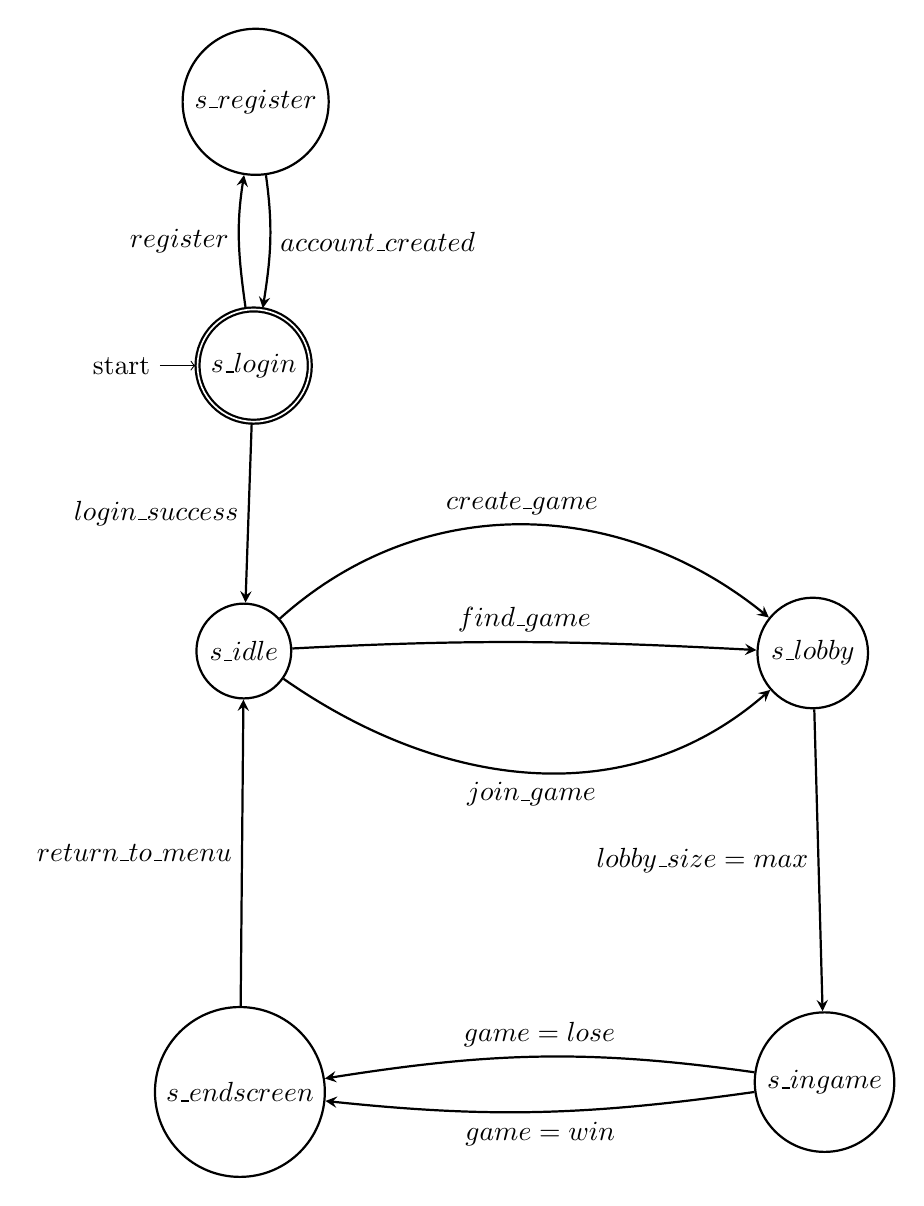
\begin{tikzpicture}[]
    \node[initial,thick,accepting,state] at (-3.9,4.175) (2a413fb1) {$s\_login$};
    \node[thick,state] at (-3.875,7.525) (291d825b) {$s\_register$};
    \node[thick,state] at (-4.025,0.55) (e39a07c9) {$s\_idle$};
    \node[thick,state] at (3.2,0.525) (981cc1fb) {$s\_lobby$};
    \node[thick,state] at (3.35,-4.925) (d4f7f4ce) {$s\_ingame$};
    \node[thick,state] at (-4.075,-5.05) (21148f7e) {$s\_endscreen$};
    \path[->, thick, >=stealth]
    (2a413fb1) edge [left,in = -99, out = 98] node {$register$} (291d825b)
    (2a413fb1) edge [left] node {$login\_success$} (e39a07c9)
    (291d825b) edge [right,in = 81, out = -82] node {$account\_created$} (2a413fb1)
    (e39a07c9) edge [above,in = 141, out = 42] node {$create\_game$} (981cc1fb)
    (e39a07c9) edge [above,in = 177, out = 3] node {$find\_game$} (981cc1fb)
    (e39a07c9) edge [below,in = -139, out = -35] node {$join\_game$} (981cc1fb)
    (981cc1fb) edge [left] node {$lobby\_size=max$} (d4f7f4ce)
    (d4f7f4ce) edge [above,in = 9, out = 172] node {$game=lose$} (21148f7e)
    (d4f7f4ce) edge [below,in = -6, out = -172] node {$game=win$} (21148f7e)
    (21148f7e) edge [left] node {$return\_to\_menu$} (e39a07c9)
    ;
\end{tikzpicture}
    \caption{Diagram for User State Finite State Machine}
    \label{fig:sm}
\end{figure}

\subsubsection{State Machine Definition}

Notation is based on standard academic conventions \cite{statemachine}.

$
\\
Let \, M = (Q, \Sigma, \delta, s, F)\\
Q = \{
    s\_login, s\_register, s\_idle, s\_lobby, s\_ingame, s\_endscreen
\}\\
\sigma = \{
    account\_created, register, login\_success, return\_to\_menu, create\_game,\\
    find\_game, join\_game, lobby\_size=max, game=lose, game=win
\}\\
\delta = \textrm{Shown in Figure \ref{fig:sm}}\\
s = s\_login\\
F = \{s\_login\}$




\subsection{Phase In Plan}
\begin{table}[h]
\begin{center}
\begin{tabular}{|c|c|}
\hline
    Priority Level & Date \\
    \hline
    0 & Nov 14th 2022 \\
    1 & Jan 7th 2022 \\
    2 & March 10th 2022 \\
    \hline
\end{tabular}
\end{center}
\caption{Phase In Plan for Functional Requirements}            

\end{table}


\section{Non-functional Requirements}

\subsection{Look and Feel Requirements}
\begin{enumerate}[label=NFR.\arabic*]
    \item The interface of the system shall be easy to read and the elements are not clumped together. \label{NFR.1}
    \item The elements on the interface shall be organized and placed in a logical way. \label{NFR.2}
\end{enumerate}

\subsection{Usability and Humanity Requirements}
\begin{enumerate}[label=NFR.\arabic*, resume]
    \item People with basic computer understanding shall be able to navigate the system. \label{NFR.3}
    \item The system shall be simple to understand and user should spend less than 5 minutes to understand what each part of the system does. \label{NFR.4}
    \item The system should be easily accessible so that the user can navigate around the system without the use of mouse. \label{NFR.5}
\end{enumerate}
\subsection{Performance Requirements}
\begin{enumerate}[label=NFR.\arabic*, resume]
    \item The system shall respond to a user's action within 2 seconds. \label{NFR.6}
    \item The system shall process and give results base on user's inputs within 10 seconds. \label{NFR.7}
    \item The system shall be operating 24 hours a day, 7 days a week. \label{NFR.8}
\end{enumerate}
\subsection{Operational and Environmental Requirements}
\begin{enumerate}[label=NFR.\arabic*, resume]
    \item The system should run on major browsers and devices that support these browsers. \label{NFR.9}
\end{enumerate}
\subsection{Maintainability and Support Requirements}
\begin{enumerate}[label=NFR.\arabic*, resume]
    \item The system shall provide the ability for developers to add questions and test cases when needed. \label{NFR.10}
\end{enumerate}
\subsection{Security Requirements}
\begin{enumerate}[label=NFR.\arabic*, resume]
    \item The system shall require users to register their own accounts in order to use the system. \label{NFR.11}
    \item The system shall deny the user access if the user fails to login. \label{NFR.12}
\end{enumerate}
\subsection{Cultural Requirements}
\begin{enumerate}[label=NFR.\arabic*, resume]
    \item The system shall not have anything that is or suggests cultural inappropriate content to society. \label{NFR.13}
\end{enumerate}
\subsection{Legal Requirements}
\begin{enumerate}[label=NFR.\arabic*, resume]
    \item The system shall be protected by GNU General Public License (GPL). \label{NFR.14}
\end{enumerate}
\subsection{Health and Safety Requirements}
\begin{enumerate}[label=NFR.\arabic*, resume]
    \item The system shall not have any flashing lights that can put the user under the risk of epilepsy or seizure. \label{NFR.15}
\end{enumerate}
% This section is not in the original Volere template, but health and safety are
% issues that should be considered for every engineering project.

\section{Traceability Table}


\begin{table}[H]
    \begin{tabularx}{\textwidth}{|p{3cm}|p{3cm}|X|}
    \hline
    Non-Functional Requirements & Functional Requirements & Rationale \\
    \hline
    \ref{NFR.1} \ref{NFR.2}  \ref{NFR.3} \ref{NFR.4}  \ref{NFR.5} \ref{NFR.15} & \ref{FR.4} \ref{FR.8} \ref{FR.16} \ref{FR.19} \ref{FR.26} \ref{FR.27} \ref{FR.28} \ref{FR.29} & Requirements that are focused on interface design requirements.\\
    \hline
    \ref{NFR.6} \ref{NFR.7}  & \ref{FR.6} \ref{FR.7} \ref{FR.14} \ref{FR.15} \ref{FR.20} \ref{FR.21} \ref{FR.22} & Requirements that are focused on performance of user experience and code compilation.  \\
    \hline
    \ref{NFR.11} \ref{NFR.12} & \ref{FR.17} \ref{FR.18} \ref{FR.19} & Requirements that are focused on account security and management\\
    \hline
    \end{tabularx}
    \caption{Traceability Table for Functional and Non-Functional Requirements}
    \label{tab:trace}
\end{table}

\section{Project Issues}

\subsection{Open Issues} 
\begin{itemize} 
    \item Judging and evaluation of a user submission
    \item Safety, managing malicious code submissions
\end{itemize}

\subsection{Off-the-Shelf Solutions}
N/A

\subsection{New Problems}
N/A

\subsection{Tasks}
\begin{itemize} 
    \item Back-end architecture design
    \item Front-end UI design
    \item Communication schema design between front-end and back-end
    \item Database schema design
    \item Unit tests for front-end and back-end
    \item End to End integration tests
\end{itemize}

\subsection{Migration to the New Product}
N/A

\subsection{Risks}
\begin{itemize}
    \item Multiple concurrent communications between front-end and back-end
    \item Back-end server may not be able to handle multiple concurrent of compilation
    \item Distributed Denial-of-Service attacks
    \item Malicious code injections
\end{itemize}

\subsection{Costs}
\begin{itemize}
    \item Back-end hosting server costs
    \item Front-end hosting server costs
    \item Database hosting costs
\end{itemize}

\subsection{User Documentation and Training}
N/A

\subsection{Waiting Room}
N/A

\subsection{Ideas for Solutions}
For concurrent communications and concurrent code compilations, vertical scaling for hardware is an easy fast method to remove the limitations of concurrency. However this leads to future higher costs. Load balancing can be used to allow for horizontal scaling of system.

For costs, many options exists for free/hobby tier project hosting, allowing for cost savings.

\newpage

\section{Appendix}

%This section has been added to the Volere template.  This is where you can place
%additional information.

\subsection{Identifying Required Knowledge}

What knowledge and skills will the team collectively need to acquire to successfully complete this capstone project? Examples of possible knowledge to acquire include domain-specific knowledge from the domain of your application, software engineering knowledge, mechatronics knowledge or computer science knowledge. Skills may be related to technology, writing, presentation, team management, etc. You should look to identify at least one item for each team member.

\begin{enumerate}

\item  \textbf{Presentation}:
Learning how to speak confidently in front of an audience allows for the best demonstration of our project. As we present our capstone, presentation skills will allow the team to reduce miscommunication and fully get our message across. Not only will this benefit the capstone project, it is a transferable skill to the real world. 

\item  \textbf{Project Management}:
Project management for a team of 5 with a large project isn't something the team is familiar with and it is key for completing our project successfully. This includes splitting off features/work among us, reviewing each other's pull requests and planning meetings or sprints.

\item \textbf{Two way web communication technology}: Learning this technology will be necessary for the success of our project as it is required to make our project collaborative. This technology will allow the project to communication between server and client and will be a key part of our project.

\item  \textbf{Continuous Integration and Continuous Delivery (CI/CD) - Zhiming Zhao}:
CI/CD connects development and operation activities together, it will enforce automation in developing, building, testing and code deployment. CI/CD compiles the incremental code changes made by developers, then package them as software deliverable. Automated tests are running constantly to verify the software functionality, and automated deployment services deliver them to end users. 

\item \textbf{System Design - Youssef Rizkalla}: 
Architecting a good design for the back-end and front-end of the system is essentially to creating a friction-less environment that allows us to fulfill and test the requirements according to their deadlines. Learning design patterns and applying them when needed will be necessary, as well as learning how to enforce coding standards when reviewing and writing code to maintain codebase health.

\end{enumerate}

\subsection{Acquiring Required Knowledge}

For each of the knowledge areas and skills identified in the previous question, what are at least two approaches to acquiring the knowledge or mastering the skill? From the identified approaches, which will each team member pursue, and why did they make this choice?

\begin{enumerate}

\item \textbf{Presentation - Dipendra Subedi} An approach to develop presentation skills is to practice speaking in front of audiences. In front of an audience, we can increase the confidence for public speaking, practice maintaining eye-contact, and speaking coherently. Another approach is to participate as a member of the audience in a presentation with great speakers. Being able to mimic exemplary presentation skills can be a guide when we are presenting ourselves. Dipendra will work on this skill as he is the design lead, so it is crucial to be able to effectively communicate ideas. When presenting the capstone project, this will also help since he will take more of a speaking role to describe the system.

\item  \textbf{Project Management - Tamas Leung}: In order to learn project management is through researching and testing out different project management strategies. This involves learning tools such as GitHub project board/kanban boards. This can be practiced by assigning priorities and weights to tasks and ensuring other teammates have a good weight of tasks per week. Tamas will work on this skill as he is the scrum lead. He will ensure that every task is on a timeline and are on track to be finished as stated on the development plan.

\item \textbf{Two way web communication technology - Anton Kanugalawattage}: This skill could be acquired by reading and following examples of existing implementation using this technology. Another approach to acquire this skill is to read the documentation or blogs of how this technology is used in systems (networking classes, technology company's engineering blogs). Anton will pursue this skill as he has worked on a project which has utilized a similar technology before. Also, as he is the front-end lead this technology will be a crucial part of the front-end and back-end integration. 

\item \textbf{CI/CD - Zhiming Zhao}: There are a lot of benefits to adapt CI/CD. First of all, there will be reduced risk on delivery. The automated tests will test the code changes before it's deployed, this will result in a higher product quality and low rates of bugs in production. The software will ship quickly and more efficiently since CI/CD pipelines move applications from coding to deployment at scale. The team will also have improved productivity since everything is moving at a faster pace.

\item\textbf{System Design - Youssef Rizkalla}: This can be developed by observing and critiquing open-source projects, as well as projects previously worked on. Youssef will work on this as he is the back-end lead and main code-reviewer. By doing this, he can identify issues that have occurred in the past and develop a design to get around them. Additionally, design patterns can be learned from official documentation or trustworthy blog posts that are published by professional Software Engineers. When reviewing code, Youssef can ensure that others are following the correct standards and design patterns. Additionally, re-iterations of the design can be done as needed if engineers feel that features are taking longer to develop and/or test than they should be.

\end{enumerate}

\subsection{Symbolic Parameters}
N/A
%The definition of the requirements will likely call for SYMBOLIC\_CONSTANTS.
%Their values are defined in this section for easy maintenance.


\begin{thebibliography}{9}
\bibitem{statemachine}
N.R. Satish, University of California, Berkeley. (n.d.). Finite State Machine. Our Pattern Language. Retrieved October 3, 2022, from \href{https://patterns.eecs.berkeley.edu/?page_id=470}{https://patterns.eecs.berkeley.edu/?page\_id=470} 
\end{thebibliography}

\end{document}
